%%%%%%%%%%%%%%%%%%%%%%%%%%%%%%%%%%%%%%%%%%%%%%%%%%%%%%%%%%%%%%%%%%%%%%%%%%%%%%
% CS110: Introduction to Computing
% Copyright 2015 Pejman Ghorbanzade <mail@ghorbanzade.com>
% Creative Commons Attribution-ShareAlike 4.0 International License
% https://github.com/ghorbanzade/UMB-CS110-2015S/blob/master/LICENSE
%%%%%%%%%%%%%%%%%%%%%%%%%%%%%%%%%%%%%%%%%%%%%%%%%%%%%%%%%%%%%%%%%%%%%%%%%%%%%%

\def \topDirectory {.}
\def \texDirectory {\topDirectory/src/main/tex}

\documentclass[12pt,letterpaper,twoside]{article}
\usepackage{\texDirectory/template/style/directives}
\usepackage{\texDirectory/template/style/assignment}
%%%%%%%%%%%%%%%%%%%%%%%%%%%%%%%%%%%%%%%%%%%%%%%%%%%%%%%%%%%%%%%%%%%%%%%%%%%%%%
% CS110: Introduction to Computing
% Copyright 2015 Pejman Ghorbanzade <mail@ghorbanzade.com>
% Creative Commons Attribution-ShareAlike 4.0 International License
% https://github.com/ghorbanzade/UMB-CS110-2015S/blob/master/LICENSE
%%%%%%%%%%%%%%%%%%%%%%%%%%%%%%%%%%%%%%%%%%%%%%%%%%%%%%%%%%%%%%%%%%%%%%%%%%%%%%

\course{id}{CS110}
\course{name}{Introduction to Computing}
\course{venue}{Tue/Thu, 5:30 PM - 6:45 PM}
\course{semester}{Spring 2015}
\course{department}{Department of Computer Science}
\course{university}{University of Massachusetts Boston}

\instructor{name}{Pejman Ghorbanzade}
\instructor{title}{}
\instructor{position}{Student Instructor}
\instructor{email}{pejman@cs.umb.edu}
\instructor{phone}{617-287-6419}
\instructor{office}{S-3-124B}
\instructor{office-hours}{Tue/Thu 19:00-20:30}
\instructor{address}{University of Massachusetts Boston, 100 Morrissey Blvd., Boston, MA}


\begin{document}

\doc{title}{Solution to Assignment 1}
\doc{date-pub}{Feb 03, 2015 at 5:30 PM}
\doc{date-due}{Feb 17, 2015 at 5:30 PM}
\doc{points}{8}

\prepare{header}

\section*{Question 1}

The code snippet below gives a Java \textit{Hello World!} program.
\lstset{language=Java}
\begin{lstlisting}
public class HelloJava {
	public static void main(String[] args) {
		System.out.println("Hello World!");
	}
}
\end{lstlisting}
As we discussed in class, Java is not the only programming language capable of such miracles. Write programs \texttt{HelloPython.py}, \texttt{HelloC.c} and \texttt{HelloPhp.php} that print \textit{Hello World!} in Python, C and Php programming languages, respectively.
\begin{figure}[H]\centering
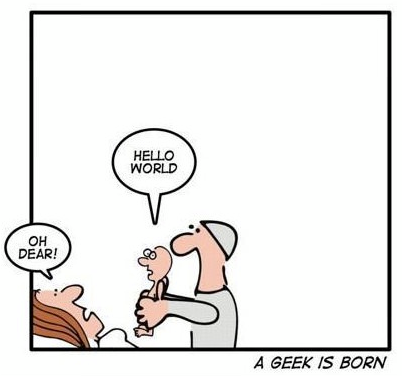
\includegraphics[width=8cm]{\texDirectory/template/images/helloworld.png}
\end{figure}
\newpage

\subsection*{Solution}

A simple \texttt{HelloPython.py} program.
\lstset{language=Python}
\begin{lstlisting}
# Comment in Python
print('Hello Python!')
\end{lstlisting}
A simple \texttt{HelloC.c} program.
\lstset{language=C}
\begin{lstlisting}
/* Comment in C */
#include<stdio.h>
int main() {
    printf("Hello C!\n");
    return 0;
}
\end{lstlisting}
A simple \texttt{HelloPhp.php} program.
\lstset{language=php}
\begin{lstlisting}
// Comment in Php
echo "Hello Php!";
\end{lstlisting}

\section*{Question 2}

Generally, a programmer's objective is to develop a program with no \textit{compilation error} that functions as originally desired, i.e. no \textit{run-time error}.
But errors occur almost inevitably during development of any program.
A reliable measure of a programmer's proficiency is how efficiently he can identify and fix his errors.
To do this, however, one must first understand the errors.

In this question, you are asked to intentionally introduce compilation errors to your \texttt{HelloWorld.java} program. Prepare a file \texttt{ErrorList.txt}, listing as many different compiler complaints as possible along with mistake(s) which cause them.

\subsection*{Solution}

Some of the compilation errors possible for a \texttt{HelloWorld.java} program in Eclipse IDE are given in Table \ref{tab1}.

\begin{table}
\begin{tabular}{|L{5cm}|L{8cm}|}
\hline
Cause & Error \\
\hline
; for print statement omitted &
Syntax error, insert ";" to complete BlockStatements\\
\hline
\{ for main method omitted &
Syntax error on token ")", \{ expected after this token\\
\hline
; replaced with \{ for main method &
This method requires a body instead of a semicolon\\
\hline
closing brace omitted & Syntax error, insert "\}" to complete ClassBody\\
\hline
both closing braces omitted & Syntax error, insert "\}" to complete MethodBody\\
\hline
closing double-quote omitted & String literal is not properly closed by a double-quote\\
\hline
starting double-quote omitted & Syntax error on token(s), misplaced construct(s) Hello cannot be resolved to a type
Syntax error on token "!", ; expected String literal is not properly closed by a double-quote\\
\hline
\texttt{println} is misspelled & The method prinsln(String) is undefined for the type PrintStream\\
\hline
one of \texttt{public}, \texttt{static}, \texttt{void}, \texttt{main}, \texttt{String[]}, \texttt{args} keywords are omitted& Main method not found in class \texttt{HelloWorld}, please define the main method as: \texttt{public static void main(String[] args)}\\
\hline
\texttt{HelloWorld} class is misspelled & Could not find or load main class \texttt{HelloWorld}\\
\hline
\end{tabular}
\caption{Compilation errors for \texttt{HelloWorld.java} program}
\label{tab1}
\end{table}

\section*{Question 3}

Write a program \texttt{Cartesian.java} that takes three command-line arguments as $X$, $Y$ and $Z$ in Cartesian coordinates and prints their corresponding $\rho$, $\theta$ and $\phi$ in Spherical coordinates.

\subsection*{Solution}
\lstset{language=Java,tabsize=2}
\begin{lstlisting}
public class Cartesian {
	public static void main (String[] args) {
		// command-line arguments are String
		// they should first be converted to double
		double x, y, z; // declaring cartesian coordinates
		x = Double.parseDouble(args[0]);
		y = Double.parseDouble(args[1]);
		z = Double.parseDouble(args[2]);
		System.out.printf("X is %.2f\n", x);
		System.out.printf("Y is %.2f\n", y);
		System.out.printf("Z is %.2f\n", z);
		// rho, phi and theta are also declared as double
		double rho, phi, theta;
		rho = Math.sqrt( Math.pow(x,2) + Math.pow(y, 2) + Math.pow(z, 2) );
		theta = Math.atan( y / x ) * 180 / Math.PI;
		phi = Math.acos( z / rho) * 180 / Math.PI;
		System.out.printf("Rho is %.3f\n", rho);
		System.out.printf("Phi is %.3f\n", phi);
		System.out.printf("Theta is %.3f\n", theta);
	}
}
\end{lstlisting}

\section*{Question 4}

Write a program \texttt{BodyMassIndex.java} that takes your weight in pounds and height in inches and calculates your Body Mass Index (BMI) according to Equation \ref{eq1}. To evaluate your BMI, program should as well indicate under which group you are classified according to Table \ref{tab2} obtained from the Department of Health and Human Services/National Institution of Health.
\begin{equation}
BMI = \frac{weightInPounds \times 703}{heightInInches^2}
\label{eq1}
\end{equation}
\begin{table}[H]\centering
\begin{tabular}{|r|l|}
\hline
Group & BMI index \\
\hline
Underweight & less than 18.5 \\
Normal & between 18.5 and 24.9 \\
Overweight & between 25 and 29.9 \\
Obese & greater than or equal to 30 \\
\hline
\end{tabular}
\caption{BMI classification}\label{tab2}
\end{table}

\subsection*{Solution}

\lstset{language=Java,tabsize=2}
\begin{lstlisting}
public class BodyMassIndex {
	public static void main (String[] args) {
		// command-line arguments are of String form
		// they should be converted to numbers
		// we convert to double to perform math calculations
		double weight = Double.parseDouble(args[0]);
		double height = Double.parseDouble(args[1]);
		System.out.printf("Weight is %.2f pounds\n",weight);
		System.out.printf("Height is %.2f inches\n",height);
		double BMI = weight * 703 / (Math.pow(height, 2));
		System.out.printf("Your BMI is %.2f\n",BMI);
		// A simple if-elseif-else loop
		String group; // we declare group in advance for better organization
		if (BMI < 18.5) {
			group = "Underweight";
		}
		else if (BMI < 24.9) {
			group = "Normal";
		}
		else if (BMI < 29.9) {
			group = "Overweight";
		}
		else {
			group = "Obese";
		}
		System.out.println("According to NIH standards,");
		System.out.println("You are " + group + "!");
	}
}
\end{lstlisting}

\section*{Question 5}

Write a program \texttt{Quadratic.java} that takes three integers $a$, $b$ and $c$ as command-line arguments and solves for $x$ with three digits of precision, the quadratic expression shown in Equation \ref{eq2}.
\begin{equation}
ax^2+bx+c=0
\label{eq2}
\end{equation}
Note that when discriminant is not negative, root(s) of a quadratic equation are obtained from Equation \ref{eq3}. When discriminant is negative, however, no real solution exists.
\begin{equation}
x = \frac{-b \pm \sqrt[2]{b^2-4ac}}{2a}
\label{eq3}
\end{equation}
Your program is expected to function as shown in following examples.

\textbf{Example:}
\begin{verbatim}
% java Quadratic 1 -2 -4
Solutions are -1.236 and 3.237
% java Quadratic 9 12 4
Solution is -0.667
% java Quadratic 3 4 2
No real-number solution exists
\end{verbatim}

\subsection*{Solution}

\lstset{language=Java,tabsize=2}
\begin{lstlisting}
public class Quadratic {
	public static void main(String[] args) {
		double a, b, c; // declaring coefficients
		// Convering command-line arguments to double
		a = Double.parseDouble(args[0]);
		b = Double.parseDouble(args[1]);
		c = Double.parseDouble(args[2]);
		// Calculating discriminant
		double discriminant = Math.pow(b, 2)-4*a*c;
		if (discriminant > 0) {
			double sol1 = (- b + Math.sqrt(discriminant))/(2*a);
			double sol2 = (- b - Math.sqrt(discriminant))/(2*a);
			System.out.printf("Solutions are %.3f and %.3f\n", sol1, sol2);
		}
		else if (discriminant == 0) {
			double sol = -b/2/a;
			System.out.printf("Solution is %.3f\n", sol);
		}
		else {
			System.out.println("No Real-number solution exists");
		}
	}
}
\end{lstlisting}

\end{document}
